%----------------------------------------------------------------------------------------
% Geometric Modeling Project
% Report LaTeX template (English)
% Interactive Graphics and Simulation Group
% University of Innsbruck
%----------------------------------------------------------------------------------------

\documentclass[11pt,a4paper]{article}

%----------------------------------------------------------------------------------------
% Include required packages
\usepackage{graphicx}
\usepackage{amsmath}
\usepackage{wrapfig}
\usepackage[english]{babel}
%\usepackage[ngerman]{babel}

\usepackage[utf8x]{inputenc}
\usepackage[T1]{fontenc}
\usepackage{float}

\usepackage[left=2.7cm, right=2.7cm, top=3cm]{geometry}

\usepackage{url}

%----------------------------------------------------------------------------------------
% Start document

\begin{document}


%----------------------------------------------------------------------------------------
% Title page
%----------------------------------------------------------------------------------------

\begin{titlepage} % User-defined title page

\begin{center}

\includegraphics[width=1.2cm]{images/uibk}

\begin{large}
Leopold-Franzens-Universität Innsbruck\\[5mm]
Institute of Computer Science\\
Interactive Graphics and Simulation Group\\[25mm]
\end{large}

{\LARGE \bf Geometric Modeling Project}

Advanced Computer Graphics WS14\\ 
Documentation\\[15mm]

Phillip Mildenberger\\
Stefan Spiss\\
Cem Okulmus\\[35mm]

advised by\\
Savoye Yann Pierre, PhD\\[10mm]

\vfill


Innsbruck, \today
\end{center}

\end{titlepage}


%----------------------------------------------------------------------------------------
% Main body
%----------------------------------------------------------------------------------------

\section{Introduction}
This is a really elegant and thoughtful introduction to our project. 
//introduce the name Lindenmayer-Systems, with abbreviation L-System. 

\section{Procedural plants using L-Systems and Turtle Graphics \newline visualisation}
Implemented by: Cem Okulmus

\subsection{Technical Overview}
The implementation consists of two parts. One is the "LSystem" class, which is
responsible for importing a set of rules that define the L-System and
consequently generating new strings that represent a word from the language the
L-System defined. This is done by applying a formal rewriting system, the nature
of which depends on the actual type of the L-System. The end result is a string that contains simple commands on how to "draw" a three-dimensional mesh.
\newline
The second part is the generation of a three-dimensional mesh of the wanted plant. This is done by a well known method of turtle graphics. This concept was explained in detail in the lecture, so only a concise summary will be given. The idea is that the "turtle" follows the list of commands sequentially and generates the mesh as it moves through space. To accommodate branching structures, as they are common in nature, a state stack is introduced, a state being the exact position and direction of the "turtle".

\subsection{Implementation Detail}

\subsubsection{L-System types}
Three basic types of L-Systems were implemented. Each of them is an extension of the former, so the L-Systems accepted by the first, would also be accepted by the second and third, and so forth. All L-Systems, like all formal languages, define an alphabet. Additionally L-Systems have a set for variables, where variables are a subset of the alphabet. The variables are the symbols which will be replaced in the production rules.

\begin{description}

\item[Deterministic and Context-free L-System]\hfill \\
This type of L-System is also known as D0L in literature. All its production rules must define a single symbol to replace, since it is  context-free and a string of its alphabet to replace it with. Depending on how often this is iterated, we will get a different word of the language, assuming a fixed starting symbol. 
\item[Stochastic and Context-free L-System]\hfill \\
This extends the previous type by allowing multiple rules for the same variable. These will be treated as possible applications. Their probability is uniformly distributed. (E.g.: Three rules means a probability of 1/3 for each of them)
\item[Stochastic and Context-sensitive L-System]\hfill \\
This extends the previous type by a, possibly empty, environment, for each variable. This restricts the rule, and will only apply it if the environment can be matched. Matches with multiple applicable rules are resolved by choosing the longest match, then the prior rule in the L-System definition, similar to an LR-Parser.
\end{description}


\begin{wrapfigure}{R}{0.5\textwidth}
  \begin{center}
    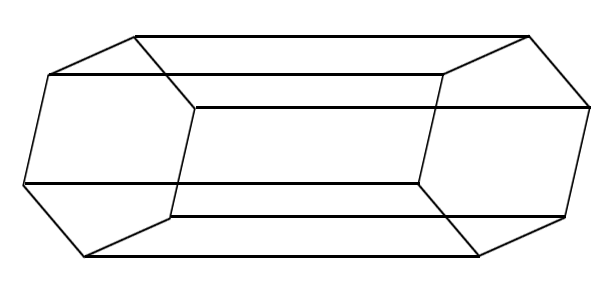
\includegraphics[width=0.45\textwidth]{images/line}
  \end{center} 
  \caption{A three-dimensional line produced by "\_3DTurtle" class}
  \label{fig:line}
\end{wrapfigure}

\subsubsection{Three-dimensional Turtle Graphics}
The "\_3DTurtle" class is very straight-forward implementation of a turtle graphics renderer in three-dimensions. The operations on meshes were implemented using OpenMesh\footnote{www.openmesh.org}, which made it very easy to add an arbitrary amount of faces to the final geometry. The needed calculations for rotation (and similar operations) in three-dimensional space were done using the library Eigen\footnote{www.eigen.tuxfamily.org}. To move in space, the three operations yaw, pitch and roll are needed to orientate the "turtle". A three-dimensional line, with a fixed length, is rendered by connecting two hexagons, as can be seen in Figure \ref{fig:line}. Additionally a polygon mode, where the turtle can sequentially follow the shape of any polygon and add it to the mesh, is provided. The interpretation of symbols is taken from a book by P.Prusinkiewicz, which also explained the Turtle Graphics model in more detail.

\section{Terrain Generation based on Stream Erosion}
Implemented by: Stefan Spiss and Phillip Mildenberger

\subsection{Technical Overview}
The project based on the paper: ``Terrain Simulation Using a Model of
Stream Erosion''\cite{kelley1988terrain}


\subsection{Implementation Detail}


\section{Results}


%----------------------------------------------------------------------------------------
% Bibliography
%----------------------------------------------------------------------------------------
\newpage
\bibliographystyle{plain}
\bibliography{EWA_literature}

\end{document}
